%\documentclass[aspectratio=43]{beamer}
\documentclass{beamer}
\usepackage[T1]{fontenc}
\usepackage[utf8]{inputenc}
\usepackage[english]{babel}
\usepackage{bm}
\usepackage{pgfplots}
\pgfplotsset{compat=newest}
\usepackage{booktabs}
%\usepackage{siunitx}
\newcommand{\Ex}{\mathbb{E}}
\newcommand{\Var}{\mathbb{V}\mathrm{ar}}
\newcommand{\Prob}{\mathbb{P}}
\DeclareMathOperator*{\argmin}{arg\,min}
% Latin Modern
%\usepackage{lmodern}
% Verdana font type
%\usepackage{verdana}
% Helvetica
%\usepackage{helvet}
% Times (text and math)
%\usepackage{newtx, newtxmath}

%\usetheme[department=compute]{DTU}
\title[Parameter control in the presence of uncertainties]{Parameter control in the presence of uncertainties} %\\ \textit{Robust Estimation of bottom friction}}
\author{\textsc{Victor Trappler} \\ AIRSEA team \\ Supervisors : Élise Arnaud, Arthur Vidard}
%\date{\today}
\titlegraphic{\includegraphics[scale= 0.38]{./Figures/MonsKlint}}
\date{27/06/2017}
\setcounter{tocdepth}{1}

\begin{document}
\frame{
	\maketitle
}

%\frame{
%	\frametitle{Outline}
%	\tableofcontents
%}
\section{Deterministic Framework}
\subsection{The 1D Shallow Water Equations}
\frame{
\frametitle{The 1D Shallow Water Equations}

	\begin{block}{1D-SWE}
		\begin{align}
			&\partial_t h + \partial_x (hu) = 0 \tag{Conservation}\\
			&\partial_t (hu) + \partial_x (u^2h + \frac{1}{2}gh^2) = -gh \partial_x Z - S \tag{Momentum}
		\end{align}
	\end{block}
%	\pause
	\begin{block}{Quadratic Friction}
	\begin{equation}
		S = - \textcolor{red}{K}\frac{|u|uh^{-\eta}}{h^2},\quad \eta = 7/3
	\end{equation}
\end{block}

}

\frame{
\frametitle{Minimization of an objective function}
We have $Y = \mathcal{H}W(K_{ref})$

\begin{equation}
\min_{K \in \mathcal{K}} j(K) = \frac{1}{2}|| \mathcal{H}W(K) - Y ||^2
\end{equation}

"Classical" optimization methods
$\rightarrow$ Adjoint-based gradient \\
But what about uncertainties due to the environment ?
}

\frame{
\frametitle{Introducing uncertainties}
$\bm{X}_e$ random vector whose realizations $\bm{x}_e$ lies in $\mathbb{X}$
\begin{equation}
    W(K) \quad \text{becomes} \quad W(\bm{x}_e,K)
\end{equation}
and the (deterministic) quadratic error is now
\begin{equation}   
   j(\bm{x}_e,K) =  \frac12||\mathcal{H}W(\bm{x}_e,K) - Y||^2
\end{equation}

%Random variable : $J(\bm{X}_e,K)$

Influence of $\bm{X}_e$ ? \\
$\argmin_K \Ex_{\bm{X_e}}[j(\bm{X}_e,K)]$ ?\\
$\argmin_K \Var_{\bm{X_e}}[j(\bm{X}_e,K)]$ ?\\

}
\frame{
\frametitle{Illustration of the robustness}
%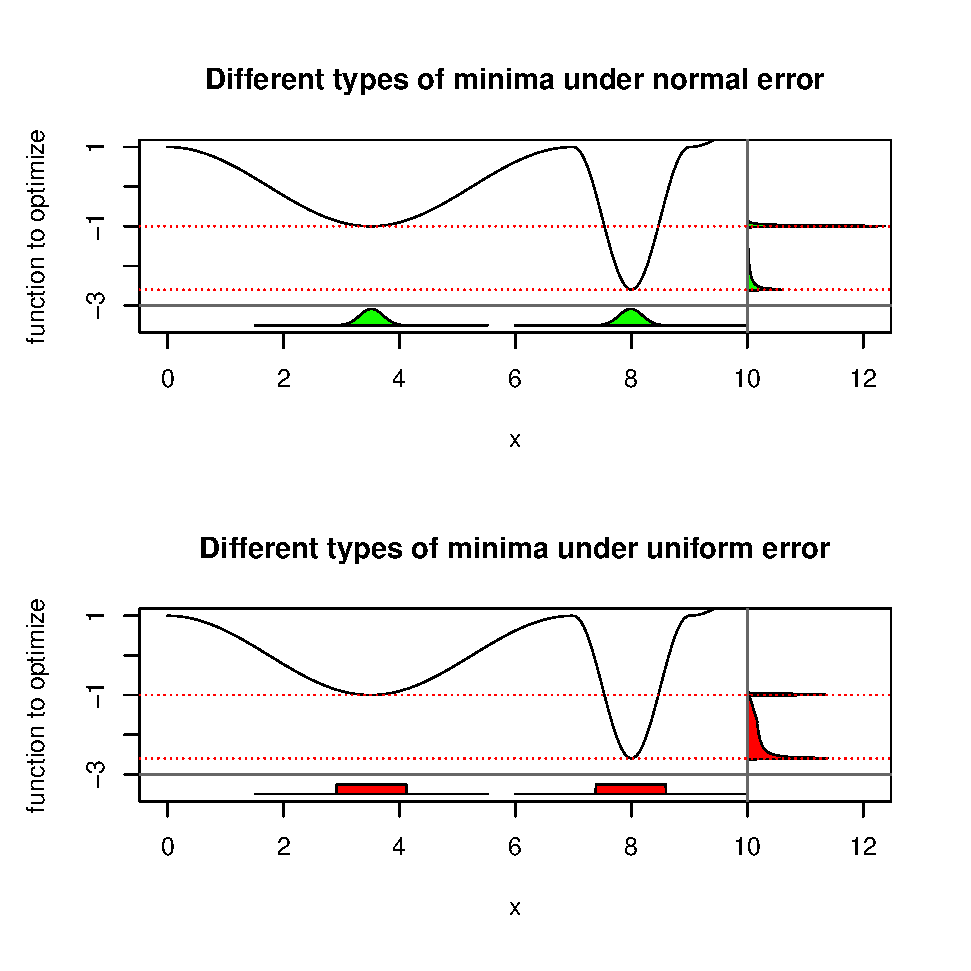
\includegraphics[scale=0.9]{./Figures/robust_2plot}
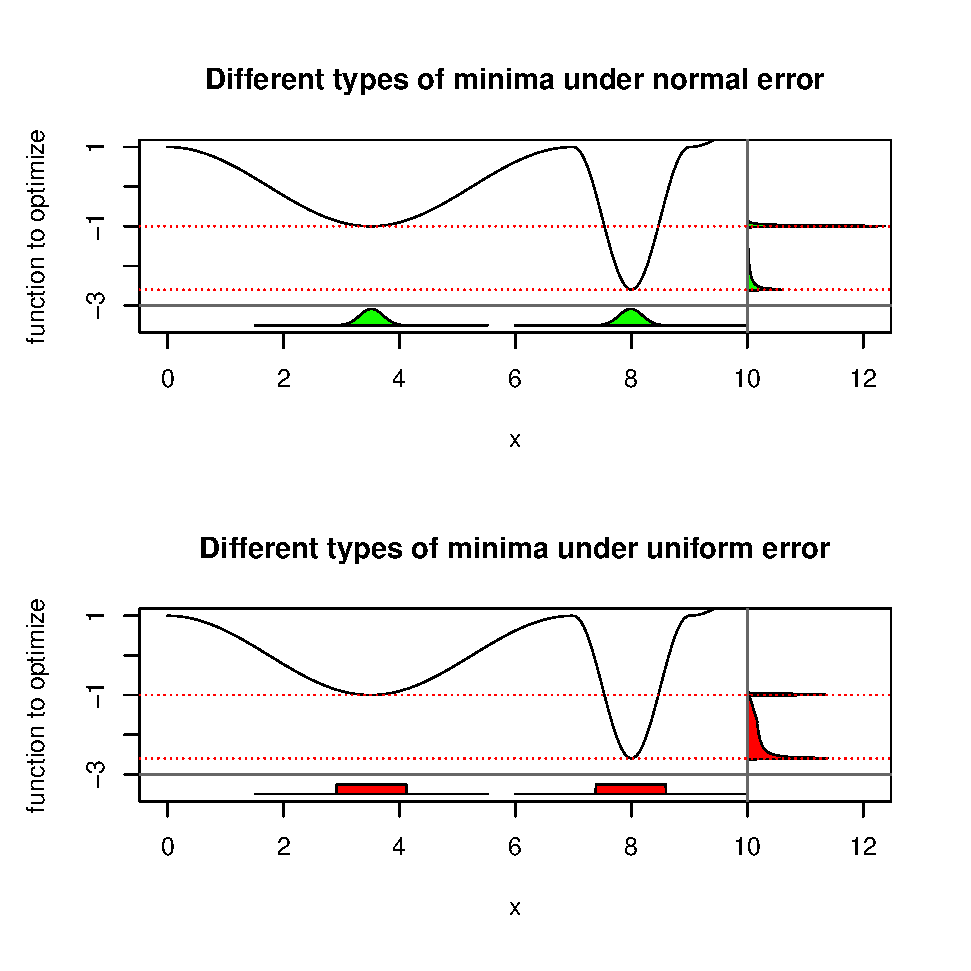
\includegraphics[trim = 0cm 0cm 0cm 8cm,clip,width = \textwidth,height = 0.7\textheight]{./Figures/robust_2plot}
}
\frame{
\frametitle{Outline of the work}
\begin{columns}[onlytextwidth]
\column{0.4\textwidth}
\begin{itemize}
\item<1-> Sensitivity analysis
\begin{itemize}
\item<1-> Sobol' indices
\end{itemize}
\item<2-> Surrogate Modelling
\begin{itemize}
\item<3-> Kriging
\item<4-> Polynomial chaos expansion
\end{itemize}
\item<5-> Robust optimization
\begin{itemize}
\item<6-> Mono objectives $\rightarrow$ M-,V-,$\rho$-robustness
\item<7-> Pareto front
\end{itemize}
\end{itemize}
\column{0.6\textwidth}
\only<3>{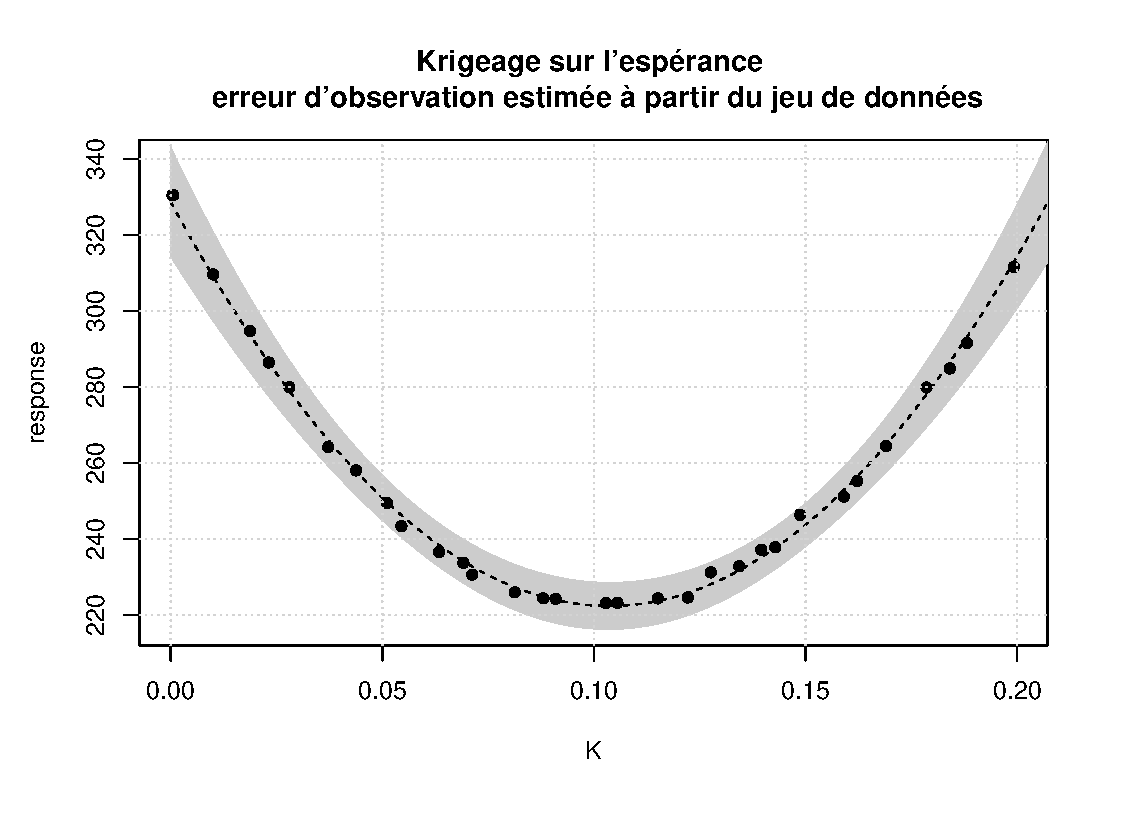
\includegraphics[width = .9\textwidth]{./Figures/krigeage_var_empirique}}
\only<4>{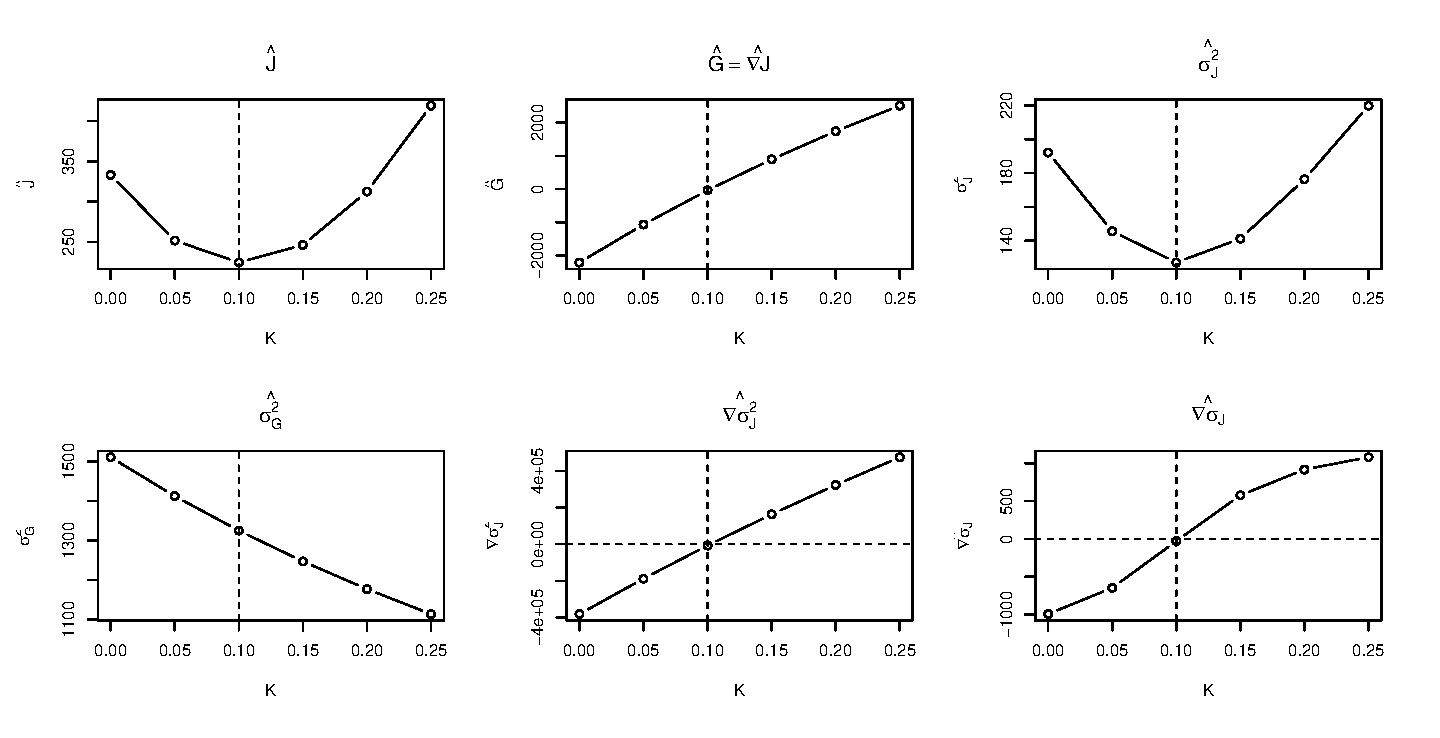
\includegraphics[width = .9\textwidth]{./Figures/PCE43}}
\only<6>{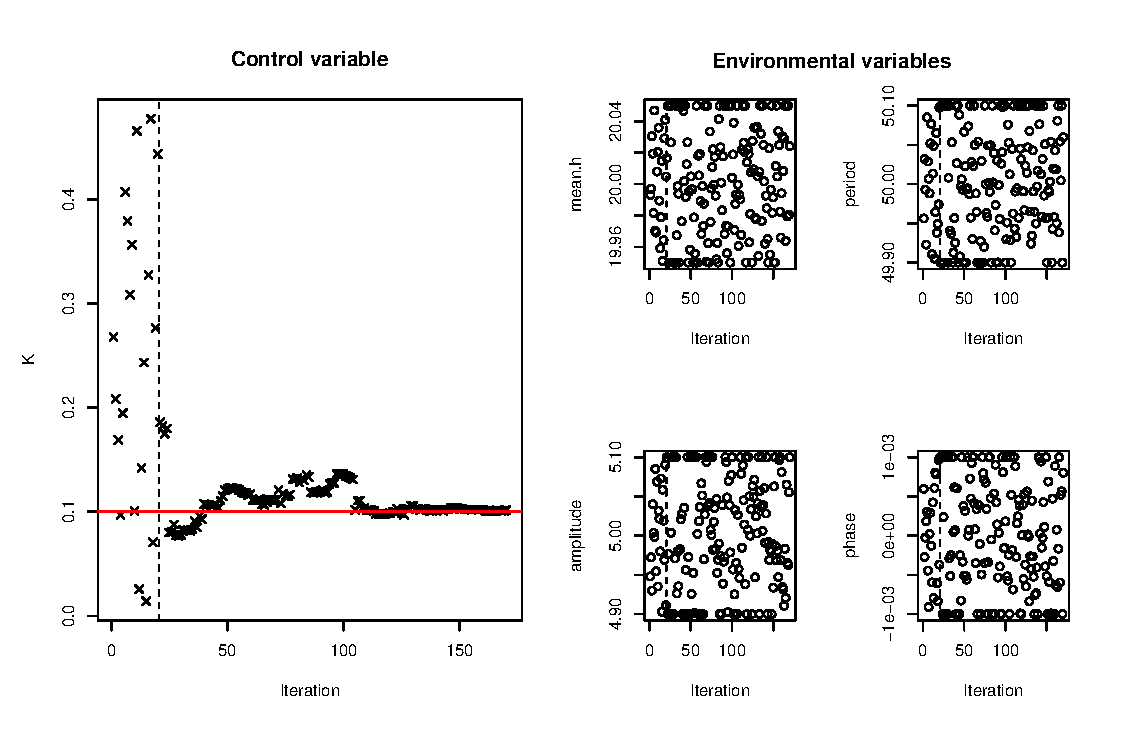
\includegraphics[width = .9\textwidth]{./Figures/exploEGO}}
\only<7>{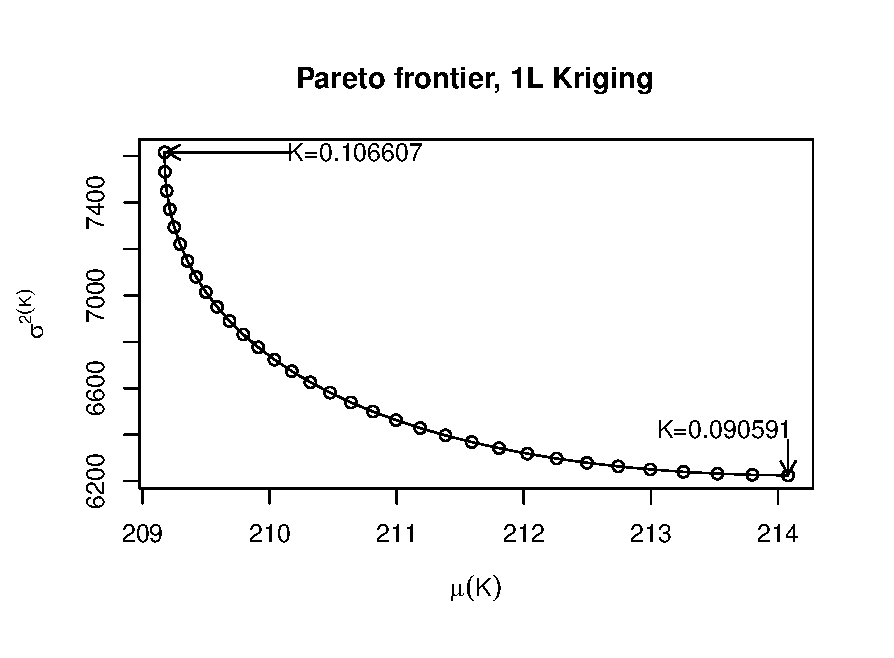
\includegraphics[width = .9\textwidth]{./Figures/pareto_1L}}
\end{columns}
}
%\subsection{Adjoint-based optimization}
%\frame{
%\frametitle{Estimation procedure, using the gradient}
%\begin{figure}[!h]
%\centering
%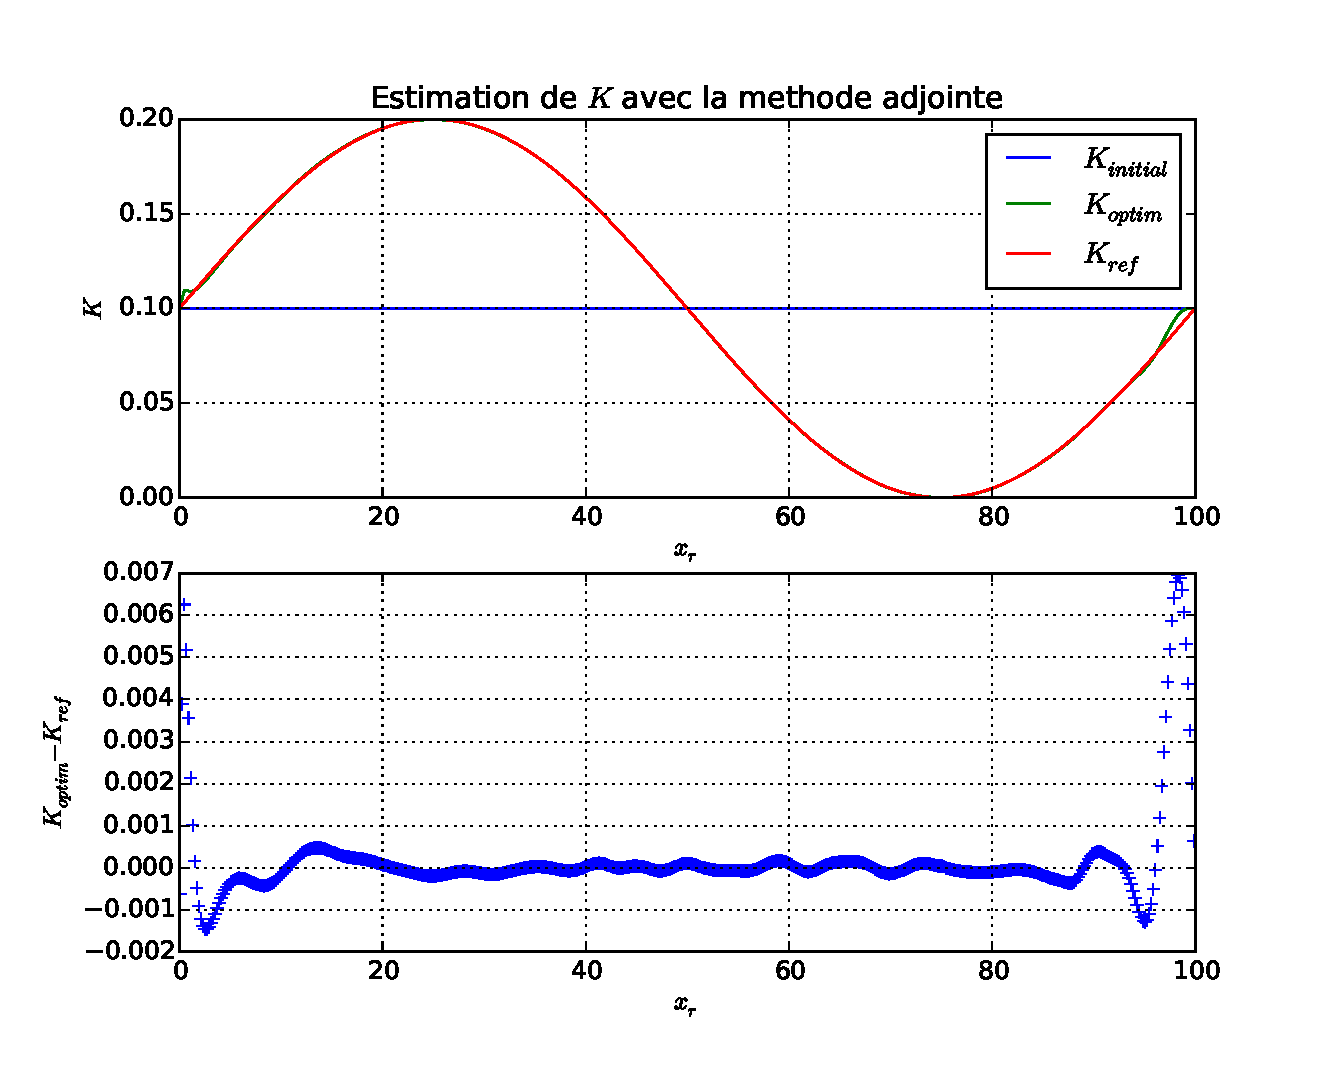
\includegraphics[width = \textwidth, height = 0.8\textheight]{./Figures/Koptim2}
%\caption{Estimation of the parameter, without uncertainties}
%\label{fig:optimdeter}
%\end{figure}
%}
%\frame{
%\frametitle{Estimation procedure, in the presence of uncertainties}
%\begin{figure}[!h]
%\centering
%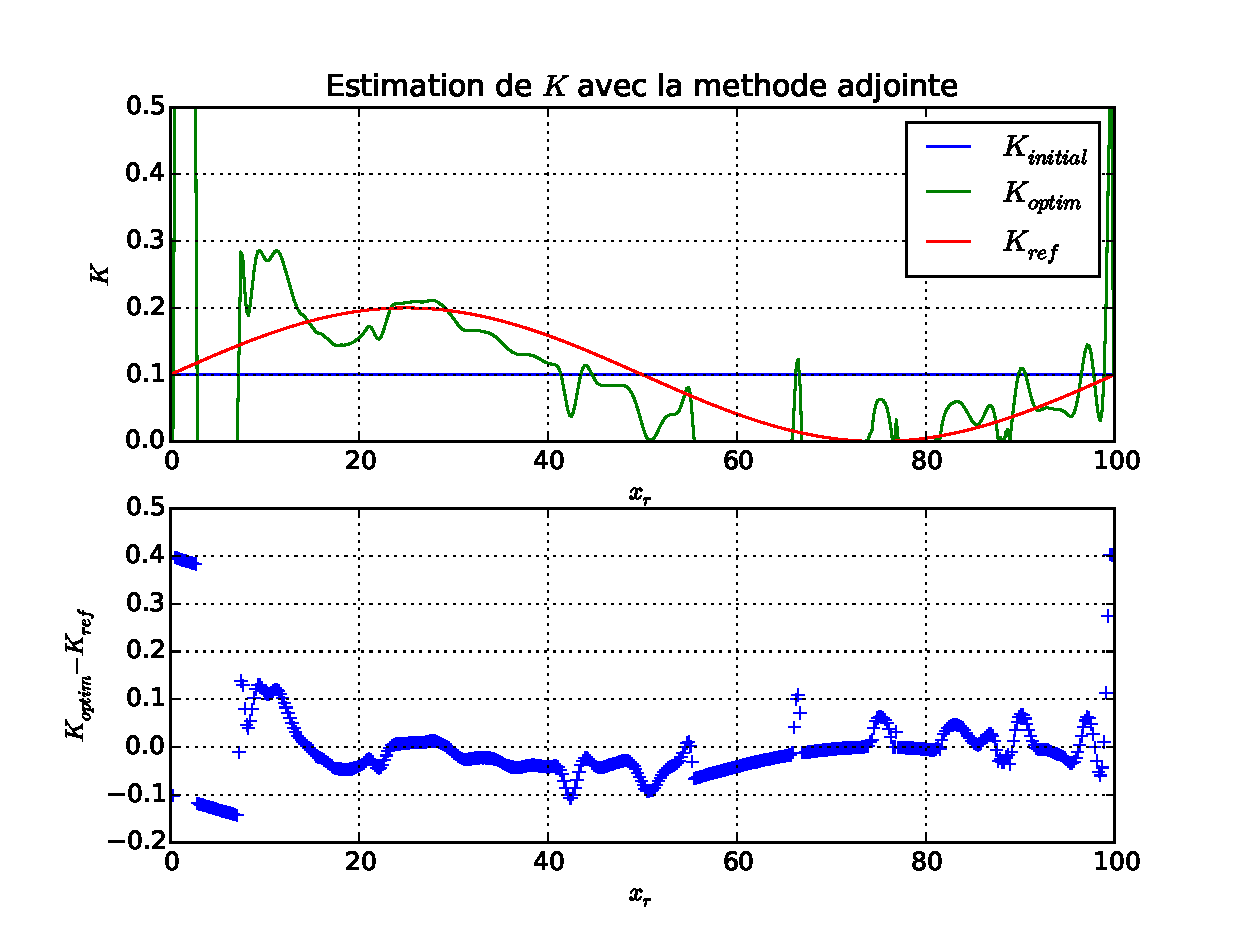
\includegraphics[width = \textwidth, height = 0.8\textheight]{./Figures/Kphaseshift}
%\caption{Estimation of the parameter, with a phase shift}
%\label{fig:optimphaseshift}
%\end{figure}
%}
%\frame{
%\frametitle{How to deal with these uncertainties ?}
%Bad estimation with just one uncertainty
%}


%\section{Metamodeling}
%\subsection{Polynomial Chaos}
%\frame{
%\frametitle{Orthogonal Polynomials in a Hilbert space}
%Decomposition on a basis of orthogonal polynomials w.r.t. a specific Kernel.
%\begin{equation}
%\langle f, g \rangle = \int_{\Omega} f(X(\omega))g(X(\omega))\, \mathrm{d}\Prob_X(\omega)
%\end{equation}
%
%\begin{equation}
%\langle f, g \rangle = \int_D f(x)g(x)w(x) \, \mathrm{d}x
%\end{equation}
%\begin{table}
%\begin{tabular}{|c|c|c|c|}
%\hline 
%Legendre & $[-1;1]$ & $w(x) = \dfrac{1}{2}$ & $\mathcal{U}([-1;1])$\\ 
%\hline 
%Hermite & $\mathbb{R}$ & $w(x) = e^{-x^2}$ & $\mathcal{N}(0,1)$ \\ \hline
%Laguerre & $[0,+\infty[$ & $w(x) = e^{-x}$ & $\mathop{Exp}$ \\ \hline
%\end{tabular} 
%\end{table}
%}
%\frame{
%\frametitle{Decomposition on a basis of orth. poly.}
%\begin{block}{Polynomial Chaos Expansion, 1D}
%	\begin{equation}
%	J(X_e,K) = \sum_{i=0}^{+\infty} \hat{J_i}(K) \varphi_i(X_e) \approx \sum_{i=0}^P \hat{J_i}(K) \varphi_i(X_e) 
%	\end{equation}
%\end{block}
%
%\begin{block}{Polynomial Chaos Expansion, multidimensional}
%	\begin{align}
%	J(\bm{X}_e,K) &= \sum_{|\bm{\alpha}|=0}^{+\infty} \hat{J_{\bm{\alpha}}}(K) \Phi_{\bm{\alpha}}(\bm{X}_e) \approx  \sum_{|\bm{\alpha}| \leq P} \hat{J_{\bm{\alpha}}}(K) \Phi_{\bm{\alpha}}(\bm{X}_e) \\
%	\bm{\alpha} &= (\alpha_1,\dots \alpha_p),\quad |\bm{\alpha}| = \sum_i \alpha_i \nonumber \\
%	\Phi_{\bm{\alpha}}(\bm{X}) &= \prod_i \varphi_{\alpha_i}(X_i) \nonumber
%	\end{align}
%\end{block}
%}
%
%\subsection{Kriging}
%\frame{
%	\frametitle{Principle of Kriging}
%	Deterministic model is a realization of a Gaussian process
%\begin{equation}
%\begin{bmatrix}
%\mathcal{J} \\
%j(x)
%\end{bmatrix} \sim \mathcal{N}\left(
%\begin{bmatrix}
%\hat{\beta}^T\mathcal{X} \\ \hat{\beta}^Tf(x)
%\end{bmatrix},
%\begin{bmatrix}
%\bm{R} & \bm{r}(x) \\
%\bm{r}^T(x) & \sigma^2
%\end{bmatrix}
%\right)
%\end{equation}
%Estimate + Variance of the predicted values
%}
%
%\section{Robust Optimization}
%\subsection{Concepts of robustness}
%\frame{
%\frametitle{Different Notions of robustness}
%\begin{itemize}
%\item<1-> M-robustness: $\min \mu(K),\quad \text{constraint on } \sigma^2(K)$
%\item<2-> V-robustness: $\min \sigma^2(K),\quad\text{constraint on } \mu(K)$
%\item<3-> $\rho$-robustness: $\min \rho(\mu(K),\sigma(K))$
%%\item<3-> $\mathcal{G}$-robustness: $\min \max_{G \in \mathcal{G}} \mu$ ,\quad $\mathcal{G}$ family of admissible distribution 
%%\item<4-> $\Pi$-robustness
%\item<4-> Multiobjective $\rightarrow$ choice within Pareto frontier.
%\end{itemize}
%}
%
%\subsection{Adaptative sampling}
%
%\frame{
%	\frametitle{Example of Optimization using Kriging and EI}
%	\begin{figure}[!h]
%	\includegraphics[width = \textwidth, height = 0.8\textheight]{./Figures/Krig_EI_exampleBIGpdf}
%	\caption{Iterative search by EI}
%	\label{fig:EIsearch}
%	\end{figure}
%}		
%%
%%\frame{
%%	\frametitle{Example of Optimization using Kriging and EI}
%%	\begin{figure}[!h]
%%	\includegraphics[width = \textwidth, height = 0.8\textheight]{./Figures/EGO1}
%%	\end{figure}
%%}
%%\frame{
%%	\frametitle{Example of Optimization using Kriging and EI}
%%	\begin{figure}[!h]
%%	\includegraphics[width = \textwidth, height = 0.8\textheight]{./Figures/EGO2}
%%	\end{figure}
%%}
%%\frame{
%%	\frametitle{Example of Optimization using Kriging and EI}
%%	\begin{figure}[!h]
%%	\includegraphics[width = \textwidth, height = 0.8\textheight]{./Figures/EGO3}
%%	\end{figure}
%%}
%%\frame{
%%	\frametitle{Example of Optimization using Kriging and EI}
%%	\begin{figure}[!h]
%%	\includegraphics[width = \textwidth, height = 0.8\textheight]{./Figures/EGO4}
%%	\end{figure}
%%}
%%\frame{
%%	\frametitle{Example of Optimization using Kriging and EI}
%%	\begin{figure}[!h]
%%	\includegraphics[width = \textwidth, height = 0.8\textheight]{./Figures/EGO5}
%%	\end{figure}
%%}
%
%\subsection{Exhaustive computation and estimation}
%\frame{
%	\frametitle{Kriging to estimate the Pareto Front}
%	Replace expensive computations by cheap computations of the metamodel
%}
%\subsection{Steepest descent}
%\frame{
%	\frametitle{Polynomial chaos for steepest descent}
%	Use of PCE to estimate $\rho$ function
%}
%\section{Conclusion}
%
%\frame{
%	\frametitle{Wrapping up}
%}
%
%\frame{
%	\frametitle{Perspective and future work}
%}
%%
%%\frame{
%%	\frametitle{Thank you for your attention}
%%	\tableofcontents
%%}

\end{document}
